%% This is an example first chapter.  You should put chapter/appendix that you
%% write into a separate file, and add a line \include{yourfilename} to
%% main.tex, where `yourfilename.tex' is the name of the chapter/appendix file.
%% You can process specific files by typing their names in at the 
%% \files=
%% prompt when you run the file main.tex through LaTeX.

\chapter{Antecedentes}

A continuación se presentan varios antecedentes de este trabajo de tesis. Primeramente se ven antecedentes generales de la computación evolutiva interactiva en la Sección \ref{cei}. En la Sección \ref{op-texto} se abarcan trabajos en donde se han enfocado en optimizar el texto publicitario encontrado en los anuncios, tal como se hace en esta tesis. En la Sección \ref{op-pos} se ven antecedentes en donde tratan la optimización publicitaria desde la perspectiva de la posición del anuncio; en otras palabras, cómo es que la posición del anuncio dentro de un sitio web afecta el rendimiento de una campaña publicitaria. En la Sección \ref{op-tipo} encontramos trabajos relacionados con la optimización del tipo de anuncio, por ejemplo, si los anuncios basados en videos son más efectivos que aquellos basados en texto o en imágenes. En la Sección \ref{rec-anuncios} se mencionan investigaciones en donde se construyen sistemas de recomendación de anuncios publicitarios. Por último, en la Sección \ref{plataformas} se presentan diversas plataformas que ayudan ya sea a la optimización de anuncios o a la recomendación de éstos.

\clearpage
\section{Optimización del Contenido en Multimedia}
\label{op-texto}

Hay diversos trabajos en donde se ha evolucionado diferentes tipos de contenidos, tales como imágenes, música, o animaciones. Sin embargo, no se encontró ninguna investigación en donde su enfoque haya sido la optimización o evolución de un texto de cualquier tipo. Aún así, muchos de estos trabajos presentan similitudes con el trabajo presentado en esta tesis, particularmente resulta de interés la forma en la que dan formato a éste contenido para que pueda ser evolucionado a través de técnicas de computación evolutiva interactiva.

\subsection{Imágenes}

Los sistemas de selección y variación por medio de recombinaciones y/o mutaciones pueden ser usados para evolucionar imágenes digitales y animaciones. La evolución interactiva puede ser usada para dirigir el desarrollo de diseños en diversas áreas de aplicación \cite{graf1995interactive}.

Dawkins \cite{dawkins1988blind} demostró el potencial de las variaciones y selección Darwinianas en los gráficos. Él evolucionó objetos gráficos bidimensionales a partir de una colección de parámetros genéticos obtenidos mediante interacciones del sistema con el usuario. Recientemente ha habido un incremento en la investigación dirigida hacia la aplicación de algoritmos genéticos a problemas relacionados con imágenes y gráficos, tales como la segmentación de imágenes de rango \cite{meygret1992robust} o identificación de patrones \cite{hill1992object}. Sims usó algoritmos genéticos para la generación interactiva de arte \cite{sims1991artificial}. Caldwell y Johnson aplicaron algoritmos genéticos para realizar búsquedas interactivas en un espacio de búsqueda de rostros de sospechosos criminales con la ayuda de testigos \cite{caldwell1991tracking}.

Picbreeder \cite{secretan2008picbreeder} es otra aplicación de la computación evolutiva para la generación interactiva de imágenes. Es un sitio web en donde los usuarios colaborativamente pueden elegir las imágenes que más les guste entre un grupo de imágenes, y éstas son usadas para obtener otras imágenes que son producto de la evolución entre las imágenes seleccionadas. Adicionalmente, Picbreeder ofrece la posibilidad de compartir imágenes entre los usuarios de su comunidad en línea, y poder continuar con la evolución de las imágenes que otros usuarios han seleccionado. También se propone un algoritmo llamado NeuroEvolución de Topologías Aumentativas (NeuroEvolution of Augmenting Topologies, o NEAT), el cual permite que los usuarios hagan estas ramificaciones de las imágenes de otros usuarios, y que puedan continuar con su evolución. Otra posibilidad ofrecida por el algoritmo NEAT es que las figuras pueden incrementarse en complejidad a través de las generaciones del proceso evolutivo.

Los objetivos que tiene Picbreeder son resolver algunos de los problemas que tiene la computación evolutiva interactiva:

\begin{itemize}
  \item Abrir la posibilidad de que grupos de individuos busquen un espacio de diseño de forma colaborativa, independientemente de sus habilidades.
  \item En la mayoría de las aplicaciones basadas en computación evolutiva interactiva los usuarios se fatigan antes de que puedan producir resultados significativos.
  \item Picbreeder promueve la proliferación del contenido. A diferencia de otros sistemas de computación evolutiva interactiva, que concentran las acciones de los usuarios en decisiones específicas, Picbreeder permite la proliferación del contenido a evolucionar.
  \item Usualmente los resultados de las evoluciones diluyen las decisiones de los usuarios, ya que estos productos son un promedio de las decisiones tomadas por todos los usuarios, y esto provoca que a ningún usuario le parezcan buenos los resultados.
  \item La plataforma promueve la participación de sus usuarios al reconocer los logros que han conseguido al estar evolucionando las imágenes. La mayoría de los sistemas similares ignoran por completo este factor.
\end{itemize}

Al permitir al usuario decidir directamente qué características dentro de los productos deberían conservarse, Picbreeder logra hacer que sus usuarios busquen dentro de un vasto espacio de diseño sin importar su talento. Los usuarios simplemente tienen que elegir qué figuras les parecen más atractivas. Debido a esta mecánica, las imágenes pueden adquirir un contenido digital complejo a causa de las decisiones invividuales de la comunidad, sin importar su nivel de experiencia.

Es muy probable que al sistema le tome muchas generaciones antes de que los usuarios comiencen a ver productos que les interese. De esta forma, la probabilidad es alta de que un usuario no encuentre algo significante dentre de las primeras 10 a 20 generaciones \cite{takagi2001interactive}, y de esta forma pierden el interés por continuar con el proceso evolutivo. Aunque el usuario mantenga el interés por muchas más generaciones, seguir buscando durante varios días puede ser demasiado tedioso. Es por esto que la fatiga en los usuarios es un problema fundamental en este tipo de sistemas. Picbreeder intenta disminuir la fatiga del usuario a través de un mecanismo llamado ramificación. Si el usuario encuentra una imagen interesante en el sitio web de Picbreeder, éste puede elegir ramificarlo, en otras palabras, puede elegir continuar con la evolución de esta imagen. De esta forma se hace más fácil lograr que una imagen se componga de cientos de generaciones logradas colaborativamente, y así los usuarios no se fatigan.

\begin{figure}[htp]
  \centerline{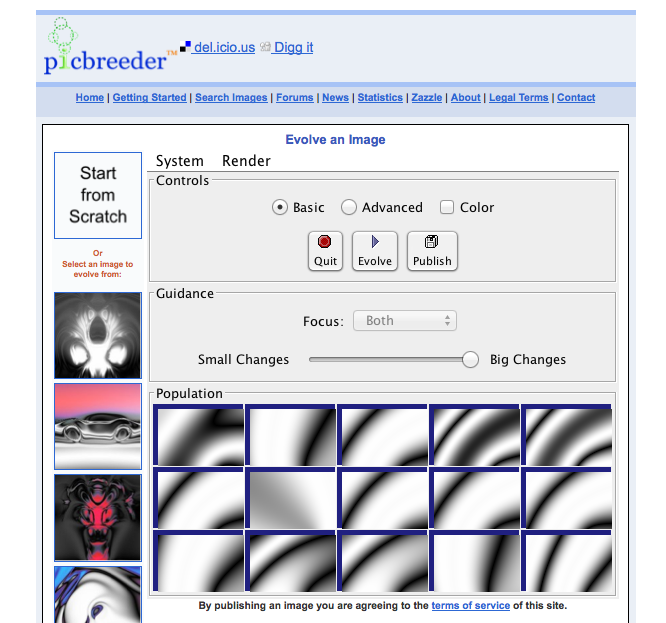
\includegraphics[width=16.09cm]{picbreeder.png}} \caption{
    Sitio web de Picbreeder, mostrando la interfaz para realizar el proceso evolutivo interactivo
} \label{Picbreeder}
\end{figure}

Otra aplicación notable en la generación de imágenes por medio de
técnicas evolutivas interactivas es EvoSpace-Interactivo. En esta
plataforma, uno puede crear aplicaciones que utilicen la computación
evolutiva interactiva. Un caso de estudio es una aplicación llamada
Fireworks \cite{trujillo2013fireworks}, la cual evoluciona animaciones artísticas y es ejecutada en
la web. Es llamada Fireworks ya que las animaciones que produce son
similares a un espectáculo de fuegos artificiales. EvoSpace
proporciona un repositorio central para la población que irá
evolucionando y para los clientes remotos, llamados EvoWorkers, los
cuales interactúan con el sistema para evaluar a los individuos usando
un enfoque interactivo.

Fireworks utiliza un lenguaje de programación llamado Processing para
codificar las animaciones artísticas, el cual facilita un desarrollo
rápido de aplicaciones gráficas para artistas y diseñadores
gráficos. El sistema promueve la colaboración de los usuarios y sus
interacciones al permitir que muchos usuarios participen en la
evaluación de los individuos en la población.

EvoSpace está basado en el modelo de espacio de tuplas, una abstacción
de Memoria Compartida Distribuída (DSM) organizada como un conjunto de
tuplas. Una tupla es el elemento básico en el espacio de tuplas,
compuesta por uno o más campos y sus valores correspondientes. En este
modelo, las operaciones básicas que puede realizar un proceso es
insertar o extraer tuplas del espacio de tuplas. EvoSpace está
compuesto por un conjunto de objetos y un conjunto de métodos de
interfaz que son dados por un servidor central. Los objetos contenidos
dentro del espacio de tuplas representan los individuos que están
evolucionando. Estos individuos están almacenados como diccionarios,
una colección de llaves únicas y valores con una asociación uno a
uno. En el servidor de EvoSpace se crea y se activa un nuevo objeto
contenedor y espera a que lleguen peticiones para ejecutar los métodos
de interfaz.

Los usuarios en Fireworks interactúan con una interfaz web. En la
Figura \ref{EvoSpace} se muestra la interfaz gráfica de EvoSpace, con
la aplicación de FireWorks. Aquí se puede ver en la parte derecha el
componente en donde se realizan las evaluaciones por parte de los
usuarios. Un usuario puede elegir una figura si le es de su agrado, y
dar clic sobre el botón de Get More. Si el usuario decide que ninguna
animación es de su agrado, puede simplemente dar clic sobre el botón
para extraer otras figuras del servidor (otra tupla del espacio de
tuplas, que con sus parámetros se genera la animación).

\clearpage

\begin{figure}[htp]
  \centerline{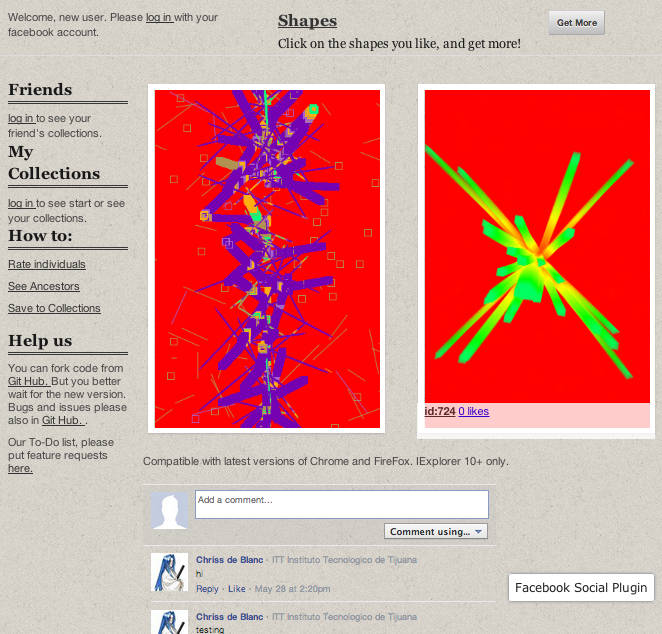
\includegraphics[width=16.09cm]{fireworks.png}} \caption{
    Sitio web de EvoSpace, mostrando la interfaz para realizar el proceso evolutivo interactivo
} \label{EvoSpace}
\end{figure}

\clearpage

Después de que el usuario termina con su interacción con los
individuos actuales, puede elegir continuar con la evolución de la
población al extraer otra muestra de EvoSpace.

Los invididuos son representados internamente como un diccionario,
como se había mencionado anteriormente. Las propiedades almacenadas
por una aplicación de EvoSpace-interactivo son una id, una cromosoma,
el número de veces que un individuo ha sido seleccionado en una
muestra y regresado a la población, los operadores genéticos que
generaron al individuo, las ids de los padres, el fitness actual, y un
diccionario de fitness.

El fitness de cada individuo es calculado basado en el número de
usuarios a los que les gustó la animación que representa, relativo al
número de veces que ha sido visto. Los usuarios sólamente pueden dar
evaluaciones positivas. Cuando un usuario evalúa una muestra de
individuos, algunos (o todos) de ellos no recibirán un voto, pero en
todos los casos la propiedad de número de vistas va a ser incrementada
en 1. Si un individuo tiene un número alto de vistas, con un número
relativamente bajo de votos, entonces este individuo es considerado
como menos apto que un individuo que tiene cerca del mismo número de
vistas y votos. Este radio de votos entre vistas es más informativo,
pero no distingue entre un individuo que tiene muchas vistas y otro
que tiene sólamente una vista, si ambos tienen cero
votos. Adicionalmente, el número de vistas debe ser mayor o igual a 1
para evitar una división entre cero.

% http://link.springer.com/chapter/10.1007/978-3-7091-6103-6_16

% @book{fels2002interactive,
%   title={Interactive, evolutionary textured sound composition},
%   author={Fels, Sidney and Manzolli, Jonatas},
%   year={2002},
%   publisher={Springer}
% }

% http://www.mitpressjournals.org/doi/abs/10.1162/096112100570602#.U-p_CYBdWDM

% @article{moroni2000vox,
%   title={Vox populi: An interactive evolutionary system for algorithmic music composition},
%   author={Moroni, Artemis and Manzolli, J{\^o}natas and Von Zuben, Fernando and Gudwin, Ricardo},
%   journal={Leonardo Music Journal},
%   volume={10},
%   pages={49--54},
%   year={2000},
%   publisher={MIT Press}
% }

% http://www.iba.t.u-tokyo.ac.jp/papers/2000/tokuiGA2000.pdf

% @inproceedings{tokui2000music,
%   title={Music composition with interactive evolutionary computation},
%   author={Tokui, Nao and Iba, Hitoshi},
%   booktitle={Proceedings of the 3rd international conference on generative art},
%   volume={17},
%   number={2},
%   pages={215--226},
%   year={2000}
% }


\clearpage
\section{Publicidad Contextual}
\label{op-pos}

La publicidad contextual es una forma de publicidad enfocada a
anuncios de sitios web y aplicaciones móviles. Estos anuncios son
seleccionados y mostrados por sistemas automatizados basados en el
contenido desplegado al usuario.

Estos sistemas están relacionados con el trabajo presentado en esta
tesis, ya que la mayor aplicación de nuestro método propuesto podría
beneficiar enormemente a las técnicas de publicidad contextual, de
forma que no sólo se elijan los mejores anuncios textuales para un
sitio web, sino que también el texto sea optimizado a lo largo del
tiempo de una campaña publicitaria.

Un sistema de publicidad contextual analiza el texto y otros elementos
de un sitio web en búsqueda de palabras clave, y muestra anuncios en
base a estas palabras clave. Estos anuncios pueden ser mostrados
dentro de la página web o dentro de otras ventanas del navegador web.

Por ejemplo, si el usuario está viendo un sitio web relacionado con
los deportes y ese sitio web usa publicidad contextual, el usuario
verá anuncios publicitarios que estén relacionado con la industria de
los deportes, tal como anuncios de compañías que venden boletos para
los partidos. La publicidad contextual también es usada por los
motores de búsqueda para desplegar anuncios en sus páginas de
resultados basándose en las palabras claves que fueron introducidas
por los usuarios.

La publicidad contextual ha tenido un gran impacto en las ganancias de
muchos sitios web. Debido a que los anuncios están enfocados, éstos
tienen una probabilidad más grande de recibir clics, y de esta forma
generan más ganancias para el dueño del sitio web. También ha recibido
gran controversia ocasionada por técnicas como los clics
automatizados, en donde aplicaciones de software dan clics
automáticamente a anuncios, así generando ganancias para el dueño de
un sitio web que fueron auto generadas.

En 2006, el total de dinero gastado en publicidad en Internet en
Estados Unidos fue de más de 17 billones de dólares, con una tasa de crecimiento de casi 20\%
cada año \cite{anagnostopoulos2007just}. Una gran parte de este
mercado consiste en anuncios textuales, en otras palabras, mensajes
cortos de texto usualmente catalogados como "enlaces destacados'' o
algo similar, dentro del sitio web. Actualmente, existen dos tipos
principales de publicidad textual en la web: búsqueda patrocinada, la
cual muestra anuncios en respuesta a las consultas en los motores de
búsqueda, y emparejamiento de contenido, el cual coloca anuncios en
sitios web.

En el trabajo propuesto por Anagnostopoulos
et. al. \cite{anagnostopoulos2007just}, se describe una solución al
problema de la publicidad contextual, en donde se utilizan técnicas de
resumen de texto, además de conocimiento externo, para realizar
resúmenes cortos de páginas web en tiempo real. Se utiliza el resumen
de texto para poder facilitar la búsqueda de los anuncios más
apropiados para los sitios web. Éstos resúmenes son producidos dentro
de los estándares de los mecanismos de JavaScript usados para el
posicionamiento de anuncios, y sólamente añaden entre 500-600 bytes a
una petición.

Además de utilizar el contenido textual en los sitios web,
Anagnostopoulos utiliza los siguientes datos para determinar qué
anuncio mostrar en el sitio web:

\begin{itemize}
  \item Utiliza la URL, separándola en palabras individuales, ya que
    es frecuente encontrar palabras significativas dentro de ésta.
  \item Además de la URL, utiliza la URL de la página que refirió a la
    página actual. Con las palabras que contiene esta URL, se puede
    saber más acerca de la intención del usuario.
  \item Se realiza una clasificación del sitio web de acuerdo a una
    taxonomía pre-establecida, y se utiliza esta categoría para ayudar
    a la determinación del anuncio a ser mostrado.
\end{itemize}

Como conocimiento externo, se utiliza una fuente usada frecuentemente \cite{brin1998anatomy}:
el texto en los enlaces que hacen referencia a la página web actual.

Otros trabajos han utilizado otras características para llevar acabo
la publicidad contextual, como en el caso del marco de trabajo
desarrollado por Fan y Chang \cite{fan2010sentiment}. Este marco de
trabajo, llamado SOCA (Sentiment-Oriented Contextual Advertising, o
Publicidad Contextual Orientada por Sentimientos), procesa el
contenido de la página web, detecta el sentimiento del contenido, y con
esto busca en una colección de anuncios para encontrar los anuncios
que sean más apropiados. Se diseñaron tres procesos para asignar los
anuncios más relevantes a una página web: un mecanismo de detección de
sentimientos, un proceso de expansión de términos, y por último, un
proceso que realiza el emparejamiento de los anuncios con las páginas
web.

Generalmente, los investigadores estudian el sentimiento en tres
niveles diferentes: nivel de palabra, nivel de enunciado, y nivel de
documento \cite{kim2004determining} \cite{kim2006automatic}. En el
trabajo de Fan y Chang, utilizaron el enunciado como la unidad mínima
e intentaron identificar aquellos enunciados que tuvieran una
opininón, y clasificaron su sentimiento en una categoría semántica
positiva o negativa usango algoritmos de aprendizaje automático y
modelos simples lineales.

\clearpage
\section{Optimización del Posicionamiento del Anuncio}

Otra característica que puede ser optimizada dentro de la publicidad
en la web, es el posicionamiento de los anuncios dentro de las páginas
web. Estos anuncios pueden estar ubicados dentro de algún menú, o
alguna otra sección o elemento dentro del sitio web, y además éstos
anuncios pueden estar ubicados en diferentes lugares en relación con
estos elementos, por ejemplo, en la parte superior del menú
izquierdo. A continuación se analizan algunos trabajos que han
estudiado esta característica de la publicidad web.

McElfresh, Mineiro y Radford \cite{mcelfresh2005method} propusieron un
método y un sistema para determinar el posicionamiento óptimo de un
anuncio en una página web, en relación a algún evento, como que el
usuario dé clic sobre estos anuncios. Para lograr esto, se
pre-establecen posiciones en la página web en donde los anuncios
pueden ser colocados. Conforme los usuarios entran al sitio web, se
recaudan datos acerca del rendimiento que han tenido los anuncios, y
nuevos datos van actualizando a los anteriores. Cuando un usuario
realiza una petición de alguna página web de este sitio, el sistema de
optimización realiza un cálculo sobre la probabilidad de que un evento
(como un clic) ocurra con cierto anuncio que es desplegado al
usuario. Todos los anuncios son ordenados de acuerdo a estas
calificaciones que obtienen con el cálculo anterior, y los que tengan
mayor probabilidad son colocados en las posiciones del sitio web.


%%%%%% Advertisement Placement

% http://www.google.com/patents/US6907566



%%%%%% Advertisement Placement





% http://www.sciencedirect.com/science/article/pii/S0925231213005110

% @article{wu2013position,
%   title={Position-wise contextual advertising: Placing relevant ads at appropriate positions of a web page},
%   author={Wu, Zongda and Xu, Guandong and Lu, Chenglang and Chen, Enhong and Zhang, Yanchun and Zhang, Hong},
%   journal={Neurocomputing},
%   volume={120},
%   pages={524--535},
%   year={2013},
%   publisher={Elsevier}
% }

% Wu, Zongda, et. al., 2013, se enfocaron en el posicionamiento óptimo de la publicidad, en lugar de la selección del anuncio para ser mostrado al usuario \cite{wu2013position}.



% http://www.gabrilovich.com/publications/papers/Anagnostopoulos2007JIT.pdf




% http://in1.csie.ncu.edu.tw/~chia/pub/SOCA.pdf




% http://people.cs.clemson.edu/~jzwang/ustc11/mm2008/p439-mei.pdf

% @inproceedings{mei2008contextual,
%   title={Contextual in-image advertising},
%   author={Mei, Tao and Hua, Xian-Sheng and Li, Shipeng},
%   booktitle={Proceedings of the 16th ACM international conference on Multimedia},
%   pages={439--448},
%   year={2008},
%   organization={ACM}
% }


% http://www.cc.ncu.edu.tw/~ncu7020/Files/Phd_Repord/98/28/thesis.pdf

% @article{fan2011blogger,
%   title={Blogger-centric contextual advertising},
%   author={Fan, Teng-Kai and Chang, Chia-Hui},
%   journal={Expert Systems with Applications},
%   volume={38},
%   number={3},
%   pages={1777--1788},
%   year={2011},
%   publisher={Elsevier}
% }


% http://www2.cse.ust.hk/~qyang/Docs/2010/vicad.pdf

% @inproceedings{chen2010visual,
%   title={Visual Contextual Advertising: Bringing Textual Advertisements to Images.},
%   author={Chen, Yuqiang and Jin, Ou and Xue, Gui-Rong and Chen, Jia and Yang, Qiang},
%   booktitle={AAAI},
%   year={2010}
% }

\clearpage
\section{Optimización del Tipo de Anuncio}
\label{op-tipo}

Los anuncios en la publicidad en Internet pueden ser de diferentes
tipos, como video, animaciones GIF, imágenes estáticas, texto, o
alguna combinación de las anteriores. En este trabajo de tesis, el
enfoque es con respecto a los anuncios de texto. Sin embargo, es
relevante ver trabajos que analizan qué tipos de textos deben ser
mostrados al usuario. Como resultado de muchos de estos trabajos, se
ha visto que al usuario le interesan más los anuncios basados en
imágenes. Sin embargo, también se ha probado que los anuncios
textuales siguen siendo importantes en la publicidad de Internet.



Zheng, Chen, y Jiang, 2012, compararon el rendimiento de anuncios con sólo texto, sólo imágenes, y texto e imágenes, y concluyeron que no hay diferencia significativa entre sus rendimientos \cite{zheng2012ontology}.

Hsieh, Yu-Chen, y Kuo-Hsiang Chen, 2011, y Lewis, Whitler y Hoeg, 2013, estudiaron cómo el tipo de contenido (videos, texto, imágenes, o una mezcla de estos tipos) de un sitio web afectan la atención de un usuario hacia los anuncios de un sitio web \cite{hsieh2011different} \cite{lewis2013customer}. 

% Finalmente, la prueba de persuación usada en este trabajo ha sido utilizada anteriormente en \cite{madera2014ad}.



% http://www.google.com/patents/US20050251444

% @misc{chan2004facilitating,
%   title={Facilitating the serving of ads having different treatments and/or characteristics, such as text ads and image ads},
%   author={Chan, Wesley and Jindal, Deepak and Patel, Amit and Ranganath, Rama and Varian, Hal},
%   year={2004},
%   month=may # "~10",
%   publisher={Google Patents},
%   note={US Patent App. 10/842,643}
% }

% http://pubsonline.informs.org/doi/abs/10.1287/isre.1040.0017

% @article{hong2004does,
%   title={Does animation attract online users’ attention? The effects of flash on information search performance and perceptions},
%   author={Hong, Weiyin and Thong, James YL and Tam, Kar Yan},
%   journal={Information Systems Research},
%   volume={15},
%   number={1},
%   pages={60--86},
%   year={2004},
%   publisher={INFORMS}
% }






\clearpage
\section{Recomendación de Anuncios Publicitarios}
\label{rec-anuncios}

La decisión de qué anuncio debe de ser mostrado en el sitio web
también puede ser determinada a través de sistemas de recomendación
basados en filtrado colaborativo, filtrado por contenido, o utilizando
técnicas alternativas que aún sean consideradas parte de sistemas
de recomendación. Esta idea es relevante para nuestro trabajo, ya que
la optimización que se realiza en el método propuesto puede verse como
una recomendación para la población con la que fueron optimizados los
textos de los anuncios publicitarios. A continuación se presentan
algunos trabajos relacionados con la recomendación de anuncios en
sitios web.

En 2007, Kazienko y Adamski propusieron la extracción de patrones de
usuario a través del uso de contenido web y técnicas de minería de uso
web, y la creación de clusters en base a esta información
\cite{kazienko2007adrosa}.


Keng y Liu, 2013, analizaron cómo es que los sitios web necesitan ser
diseñados de acuerdo a la personalidad de los usuarios y sus intereses
\cite{keng2013can}.



% http://skillupjapan.co.jp/news/rd_product/pdf/2_CSCWD2010.pdf

% @inproceedings{konow2010recommender,
%   title={Recommender System for contextual advertising in IPTV scenarios},
%   author={Konow, Roberto and Tan, Wayman and Loyola, Luis and Pereira, Javier and Baloian, Nelson},
%   booktitle={Computer Supported Cooperative Work in Design (CSCWD), 2010 14th International Conference on},
%   pages={617--622},
%   year={2010},
%   organization={IEEE}
% }


% http://dspace.kaist.ac.kr/bitstream/10203/5362/1/2006-063.pdf

% @inproceedings{ahn2006mobile,
%   title={Mobile advertisement recommender system using collaborative filtering: Mar-cf},
%   author={Ahn, H and Kim, K-j and Han, I},
%   booktitle={Proceedings of the 2006 conference of the Korea society of management information systems},
%   year={2006}
% }

% http://www.researchgate.net/publication/227121110_An_efficient_ad_recommendation_system_for_TV_programs/file/e0b4952c4f95a7589d.pdf

% @article{velusamy2008efficient,
%   title={An efficient ad recommendation system for TV programs},
%   author={Velusamy, Sudha and Gopal, Lakshmi and Bhatnagar, Shalabh and Varadarajan, Sridhar},
%   journal={Multimedia Systems},
%   volume={14},
%   number={2},
%   pages={73--87},
%   year={2008},
%   publisher={Springer}
% }

% http://www.kbs.uni-hannover.de/Lehre/pers12/readingmaterial/07_pazzani-content-based-recommender-systems.pdf

% @incollection{pazzani2007content,
%   title={Content-based recommendation systems},
%   author={Pazzani, Michael J and Billsus, Daniel},
%   booktitle={The adaptive web},
%   pages={325--341},
%   year={2007},
%   publisher={Springer}
% }

% http://www.im.ethz.ch/publications/080910_PC_RecommedationSystem_FvR.pdf

% @inproceedings{von2009mobile,
%   title={A mobile product recommendation system interacting with tagged products},
%   author={Von Reischach, Felix and Guinard, Dominique and Michahelles, Florian and Fleisch, Elgar},
%   booktitle={Pervasive Computing and Communications, 2009. PerCom 2009. IEEE International Conference on},
%   pages={1--6},
%   year={2009},
%   organization={IEEE}
% }

% http://www.google.com/patents/US5774170

% @misc{alison1998system,
%   title={System and method for delivering targeted advertisements to consumers},
%   author={Alison, Tom and Beauregard, Robert G and Ciciora, Walter S and Hite, Kenneth C and others},
%   year={1998},
%   month=jun # "~30",
%   publisher={Google Patents},
%   note={US Patent 5,774,170}
% }

% http://www.google.com/patents/US20080126176

% @misc{iguchi2007user,
%   title={User-profile based web page recommendation system and user-profile based web page recommendation method},
%   author={Iguchi, Makoto},
%   year={2007},
%   month=jun # "~29",
%   publisher={Google Patents},
%   note={US Patent App. 11/772,071}
% }



% \clearpage
% \section{Marcos de Trabajo o Plataformas}
% \label{plataformas}

% Fan, Teng-Kai, y Chia-Hui Chang, 2011, propusieron un marco de trabajo de software para analizar el contenido de blogs, determinar el tema de su contenido, y recomendar anuncioos que fueran relevantes de acuerdo al contenido del blog \cite{fan2011blogger}.

% Dao, Tuan Hung, Seung Ryul Jeong, y Hyunchul Ahn, 2012, desarrollaron una herramiento que recomienda anuncios de acuerdo al contexto de un individuo. Usan la locación del usuario para proveer mejores anuncios. Su sistema de recomendación está basado en filtrado colaborativo \cite{dao2012novel}.


% http://jiad.org/download2dc4.pdf?p=13

% @article{lombard2001interactive,
%   title={Interactive advertising and presence: a framework},
%   author={Lombard, Matthew and Snyder-Duch, Jennifer},
%   journal={Journal of Interactive Advertising},
%   volume={1},
%   number={2},
%   pages={56--65},
%   year={2001},
%   publisher={Taylor \& Francis}
% }

% http://www-scf.usc.edu/~csci572/papers/Aggarwal_Framework.pdf

% @incollection{aggarwal1998framework,
%   title={A framework for the optimizing of WWW advertising},
%   author={Aggarwal, Charu C and Wolf, Joel L and Philip, S Yu},
%   booktitle={Trends in Distributed Systems for Electronic Commerce},
%   pages={1--10},
%   year={1998},
%   publisher={Springer}
% }

% http://ieeexplore.ieee.org/xpl/login.jsp?tp=&arnumber=663397&url=http%3A%2F%2Fieeexplore.ieee.org%2Fxpls%2Fabs_all.jsp%3Farnumber%3D663397

% @inproceedings{gallagher1997framework,
%   title={A framework for targeting banner advertising on the Internet},
%   author={Gallagher, Katherine and Parsons, Jeffrey},
%   booktitle={System Sciences, 1997, Proceedings of the Thirtieth Hawaii International Conference on},
%   volume={4},
%   pages={265--274},
%   year={1997},
%   organization={IEEE}
% }

% http://www.tandfonline.com/doi/abs/10.1080/0267257X.1996.9964451#.U-sNuoBdWDM

% @article{morgan1996internet,
%   title={An internet marketing framework for the World Wide Web (WWW)},
%   author={Morgan, Robert F},
%   journal={Journal of Marketing Management},
%   volume={12},
%   number={8},
%   pages={757--775},
%   year={1996},
%   publisher={Taylor \& Francis}
% }


% http://www.google.com/patents/US6714975

% @misc{aggarwal2004method,
%   title={Method for targeted advertising on the web based on accumulated self-learning data, clustering users and semantic node graph techniques},
%   author={Aggarwal, Charu Chandra and Wolf, Joel Leonard and Yu, Philip Shi-lung},
%   year={2004},
%   month=mar # "~30",
%   publisher={Google Patents},
%   note={US Patent 6,714,975}
% }
